\chapter{Rectangular Waveguide (2)}

We are investigating the propagation of electromagnetic waves inside a hollow pipe with a rectangular cross-section. We called this structure a rectangular waveguide. We had the structure for a rectangular waveguide shown below. With energy flowing along the length of the pipe. The coordinate axis is oriented in the direction shown with $a\geq b$.
\begin{figure}[h]
\centering
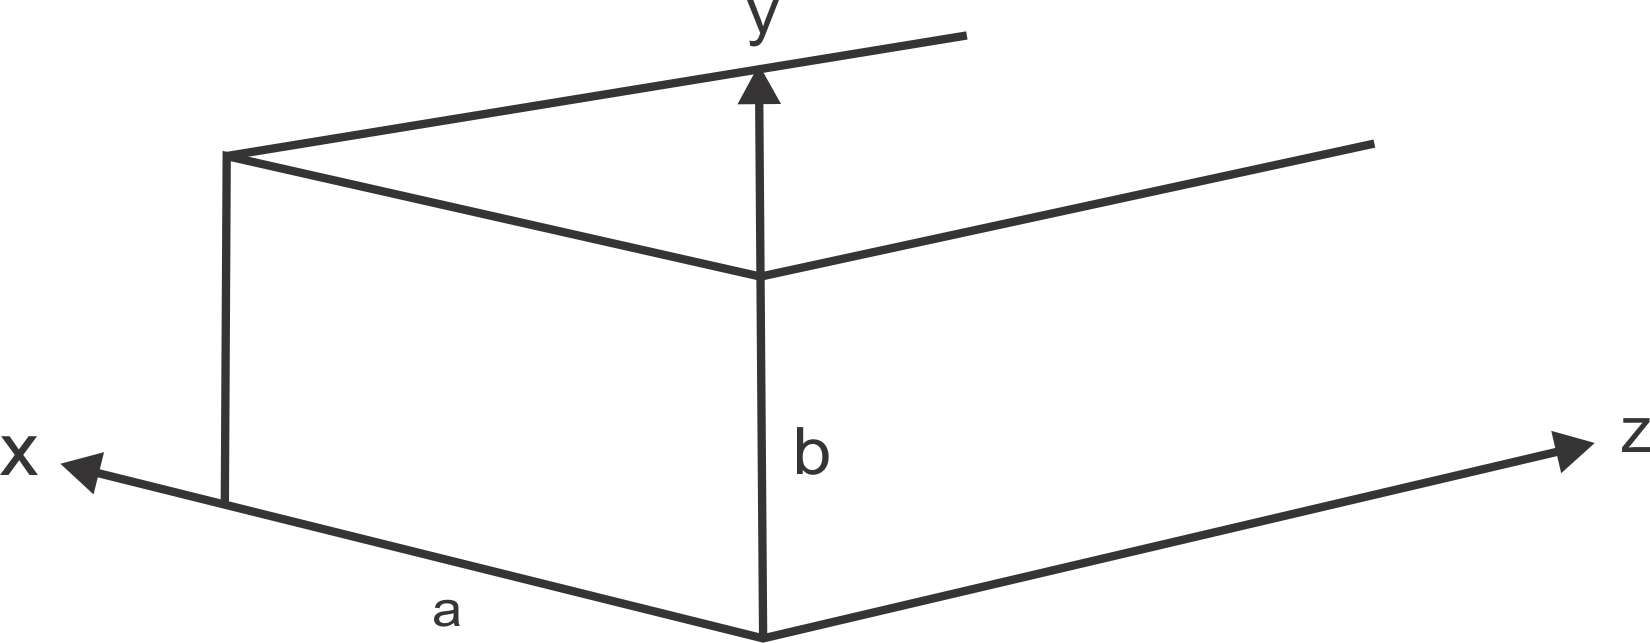
\includegraphics[width=1\linewidth]{\pathtoparttwo/graphics/group39}
\caption{A rectangular waveguide with $a>b$}
\end{figure}

\section{Transverse Electric  (TE) mode}\index{transverse electric mode}
For the transverse electric mode, we had $E_z = 0$, $H_z \neq 0$ and by comparison we had 
\begin{dmath}
H_z = C\cos(\frac{m\pi x}{a}) \cos(\frac{n\pi y}{b})e^{-j\beta z}
\label{eqn:magneticfield}
\end{dmath}

Like the case of the transverse magnetic, we denote this by TE$_{mn}$ to show the order of the transverse electric mode. We ask what are indexes required for the existence of these fields. If $m = n = 0$ i.e $\text{TE}_{00},H_z$ is not zero unlike the TM$_{00}$ mode. Recall that the transverse fields from equations~\ref{eqn:transverseex}-\ref{eqn:transversehy} expressed as:
\begin{align*}
E_x = -\frac{j\omega u}{h^2}\frac{\partial H_z}{\partial y} - \dfrac{j\beta}{h^2}\frac{\partial E_z}{\partial x}\\
E_y = \frac{j\omega u}{h^2}\frac{\partial H_z}{\partial x} - \dfrac{j\beta}{h^2}\frac{\partial E_z}{\partial y}\\
H_x = \frac{j\omega \epsilon}{h^2}\frac{\partial E_z}{\partial y} - \dfrac{j\beta}{h^2}\frac{\partial H_x}{\partial x}\\
H_y = -\frac{j\omega \epsilon}{h^2}\frac{\partial E_z}{\partial x} - \dfrac{j\beta}{h^2}\frac{\partial H_z}{\partial y}
\end{align*}
All the transverse fields involve space derivation, $\dfrac{\partial}{\partial x}$ or $\dfrac{\partial}{\partial y}$. So having a field which does not vary as a function of space $(x,y)$ for TE$_{00}$, $H_z = Ce^{-j\beta z}$  $\dfrac{\partial H_z}{\partial x}$,  $\dfrac{\partial H_z}{\partial y} = 0$ and $E_z = 0$. So that $E_x, E_y, H_x$ and $H_y$ will all go to zero. So if $m = n = 0, H_z = C \Rightarrow E_\bot , H_\bot = 0$. This means that in this situation of $m = n = 0$ for TE, we have magnetic field $H_z = Ce^{-j\beta z}$ but no electric field. What we have seen for a time-varying field is such that this can't happen as electric and magnetic fields are coupled. So if the electric field goes to zero, then the magnetic field must go to zero. This means that the constant $C$ is $H_z = Ce^{-j\beta z}$ must be identically equal to zero. This means that mode TE$_{00}$ cannot exist like TM$_{00}$.

Let's consider $H_z$ from equation~\ref{eqn:magneticfield} when $m$ or $n = 0$,
\begin{dmath*}
H_z = C \cos \left(\frac{m\pi x}{a}\right)\cos\left(\frac{n\pi y}{b}\right)e^{-j\beta z} = C \cos \left(\frac{n\pi y}{b}\right)e^{-j\beta z} \neq 0 
\end{dmath*}
or 
\begin{dmath*}
H_z = C \cos \left(\frac{m\pi x}{a}\right)e^{-j\beta z} \neq 0 
\end{dmath*}
That means TE$_{0n}$ or TE$_{m0}$ does not exist. The TE$_{0n}$ meant that the field has variation in the y-direction and TE$_{m0}$ meant that the field has variation in the x-direction but no variation in the y-direction. Hence the lowest order modes for TE mode will be TE$_{10}$ or TE$_{01}$ compared to TM$_{11}$ in TM mode. 

\section{Phase Constant}\index{phase constant}
Using a similar analysis to the TM mode, it can be shown that 
$$
\text{The wave number, }h^2 =\left(\dfrac{m\pi}{a}\right)^2 + \left(\dfrac{n\pi}{b}\right)^2
$$
and then we get phase constant in the z-direction as 
\begin{dmath*}
\bar{\beta} = \sqrt{\omega^2\mu\epsilon - h^2}
= \sqrt{\omega^2\mu\epsilon-\left(\dfrac{m\pi}{a}\right)^2- \left(\dfrac{n\pi}{b}\right)^2}
\end{dmath*}
$\bar{E},\bar{H}\sim e^{-j\beta z}$ i.e $\bar{E}\ and\ \bar{H}$ has a variation with $e^{-j\beta z}$. To show the travelling $\omega^2\mu\epsilon < \left[\left(\dfrac{m\pi}{a}\right)^2 + \left(\dfrac{n\pi}{b}\right)^2\right]$, then the phase constant becomes imaginary. At this point $e^{-j\beta z}$ does not represent a travelling wave, but exponentially decaying fields in the z-direction and the wave propagation cases.

Hence we see that the frequency must have certain values so that $\beta$ is a real quantity. That frequency as we saw in a parallel plane waveguide where the transition takes place from wave to decaying field is the cut-off frequency of the mode. So far different values of $m$ and $n$ will have different cut-off frequencies. 

\section{Cut-off Frequencies}
At cut-off frequency ${\omega_c}^2\mu\epsilon = \left(\dfrac{m\pi}{a}\right)^2 + \left(\dfrac{n\pi}{b}\right)^2$
\begin{dmath}
f_c = \frac{1}{2\pi \sqrt{\mu\epsilon}}\left[\left(\frac{m\pi}{a}\right)^2 + \left(\dfrac{n\pi}{b}\right)^2\right]^{\frac{1}{2}}
\label{eqn:cut-off}
\end{dmath}
Now knowing the order $m$ and $n$, and the dimension of the waveguide, we can determine the cut-off frequency for a particular mode.
\begin{dmath*}
\bar{\beta} = \sqrt{{\omega}^2\mu\epsilon-{\omega_c}^2\mu\epsilon}
\end{dmath*}
since ${\omega_c}^2\mu\epsilon = \left(\dfrac{m\pi}{a}\right)^2 + \left(\dfrac{n\pi}{b}\right)^2$
\begin{dmath*}
\bar{\beta} = \sqrt{\omega^2\mu\epsilon\left(1 - \frac{\omega_c^2}{\omega^2}\right)}
= \omega\sqrt{\mu\epsilon}\sqrt{1 - \frac{\omega_c^2}{\omega^2}}
\end{dmath*}
\begin{dmath*}
\bar{\beta} = \omega\sqrt{\mu\epsilon}\sqrt{1 - \left(\frac{f_c}{f}\right)^2}
\label{eqn:phaseconstrec}
\end{dmath*}
Now, this is the phase constant for the waveguide in the z-direction. Now we imagine we have this structure for which the quantity we had to measure was the variation of the electric field along the length, say we take a probe to measure the field along the length, you will observe a separation distance between two consecutive maxima that is related to the phase constant of the wave along the direction of the waveguide $\dfrac{2\pi}{\lambda}$ is what we will measure in this waveguide. This $\lambda$ is what the wave has intrinsically in an unbound medium.

For our case, let's say $\beta = \dfrac{2\pi}{\lambda}$, $\lambda$ is not the wavelength in unbound medium $\frac{c}{f}$, so we are better off saying  $\beta = \dfrac{2\pi}{\lambda_g}$. ${\lambda_g}$ best describes the distance between two maxima of the electric field that we would measure inside the rectangular waveguide. So $\lambda$ is the intrinsic wavelength\index{intrinsic wavelength} of the wave in an unbound medium $\dfrac{c}{f}$, inside the wavelength we have a modified wavelength to $\lambda_g$ which is related to $\lambda$. So $\lambda g$ is the wavelength for the guided electric and magnetic field distribution inside the rectangular waveguide and it is called the \textbf{Guide Wavelength}\index{guide wavelength}. 

\section{Guide Wavelength}
$\beta$ is the phase constant we measured as we move the probe along to get successive maxima inside the waveguide.$\lambda$ is not what we measure along the waveguide but $\lambda_g$

From equation~\ref{eqn:phaseconstrec}, $\beta$ is related to  $\beta = \dfrac{2\pi}{\lambda_g}$, then 
\begin{dmath}
\lambda_g = \frac{\lambda}{\left[1-{\left(\frac{fc}{f}\right)}^2\right]^{\frac{1}{2}}}
\label{eqn:lambdag}
\end{dmath}
where $\lambda$ is the wavelength of the wave in unbound medium $\lambda_g$ is the wavelength that we will measure inside the bound structure along the waveguide. For travelling wave $f>f_c$ otherwise $\lambda$ is a complex number that results in exponentially decaying fields. So $\left[1-{\dfrac{fc}{f}}\right]^{\frac{1}{2}}$ is always going to be less than 1. This means $\lambda_g>\lambda$. Hence guided wavelength is always greater than the intrinsic wavelength of the medium. As $f\longrightarrow0$, $\dfrac{f_c}{f}\longrightarrow0$ at that time, $\lambda_g\longrightarrow\lambda$ but never become $\lambda$ because we would always have a finite frequency. So for a guided structure, no matter what frequency we operate at $\lambda_g>\lambda$.

Secondly, as $f\longrightarrow f_c$, when $f=f_c$, $\lambda_g = \dfrac{\lambda}{0} = \infty$ so $\lambda_g\longrightarrow\infty$ when $f\longrightarrow f_c$. We know that phase velocity $V_\rho = \dfrac{\omega}{\beta}$. When $f\gg f_c$, $V_\rho\approx c$ (intrinsic velocity) and when $f\longrightarrow f_c$, $V_\rho\longrightarrow\infty$ or if $\lambda_g\longrightarrow\infty$ because $f\longrightarrow f_c$, velocity = $\lambda_gf\longrightarrow\infty$.

These are certain important conclusions we can draw from our analysis and try to investigate the cut-off frequencies for different modes. Comparing the lowest modes for the TE and TM modes, which are TE$_{10}$, TE$_{01}$, and TM$_{11}$.
From equation~\ref{eqn:cut-off} for  $m=1$ and $n=0$, TE$_{10}$ have 
\begin{dmath*}
f_{c_{\text{TE}_{10}}} = \frac{1}{2\pi \sqrt{\mu\epsilon}}\frac{\pi}{a} = \frac{\frac{\pi}{a}}{2\pi \sqrt{\mu\epsilon}}
\end{dmath*}
for $m=0$ and $n=1$
\begin{dmath*}
f_{c_{TE{01}}} = \frac{1}{2\pi \sqrt{\mu\epsilon}}\frac{\pi}{b} = \frac{\frac{\pi}{a}}{2\pi \sqrt{\mu\epsilon}}
\end{dmath*}
for $m=1$ and $n=1$, 
\begin{dmath*} 
f_{c_{TM{11}}} = \frac{1}{2\pi \sqrt{\mu\epsilon}}\left[\left(\frac{\pi}{a}\right)^2 + \left(\dfrac{\pi}{b}\right)^2\right]^{\frac{1}{2}} = \frac{\left[\left(\frac{\pi}{b}\right)^2 + \left(\frac{\pi}{b}\right)^2\right]^{\frac{1}{2}}}{2\pi \sqrt{\mu\epsilon}}
\end{dmath*}
Recall by definition that $a>b$, for a square waveguide $a=b$. For a rectangular waveguide with $a>b$, $f_{c_{TE{10}}}$ is less than $f_{c_{TE{01}}}$ and they are both smaller than $f_{c_{TM{11}}}$. So in general, the three lowest modes for TE and TM have the relationship 
\begin{align*}
f_{c_{TE{10}}}<f_{c_{TE{01}}}<f_{c_{TM{11}}}
\end{align*}
As we have seen TE$_{00}$ or TM$_{00}$ do not exist so $f_{c_{TE{10}}}$ is the lowest frequency which can propagate on the rectangular waveguide structure. That is the absolute minimum frequency that the structure will support so whenever we try to excite a rectangular waveguide, the possibility of exciting the TE$_{10}$ mode is highest because if the wave is going to propagate at all, it will be propagating in the frequency around $f_{c_{TE{10}}}$. If the frequency lies between $f_{c_{TE{10}}}$ and $f_{c_{TE{01}}}$, it is likely TE$_{10}$ will propagate. If it lies within $f_{c_{TE{01}}}$ and $f_{c_{TM{11}}}$, it is possible  $f_{c_{TE{10}}}$ and $f_{c_{TE{01}}}$ will propagate and $f_{c_{TM{11}}}$ will not propagate. $f_{c_{TE{10}}}$ is the lowest frequency that the waveguide is capable of supporting. This is the reason the TE$_{10}$ mode is called the \textbf{Dominant mode}\index{dominant mode} of a rectangular waveguide, TE$_{10}$ mode means there is one half-cycle variation in the x-axis and no variation on the y-axis. Since it is the dominant mode, we can have a detailed analysis of this mode rather than talking about the general mode of TE$_{mn}$ or TM$_{mn}$, since if at all energy is going to propagate, it is going to be propagated in this mode depending upon the value of a and b. It is possible that the TE$_{01}$ mode may have a frequency lower than or higher than TE$_{20}$ mode or TE$_{30}$ mode lower than the TE$_{11}$ mode or TM$_{11}$ mode. So depending upon the dimension, the ratio of a and b, it is possible that a higher order TE mode like TE$_{20}$ or TE$_{30}$ may have a cut-off frequency smaller than TM$_{11}$ or they may have frequency more than that. So one cannot make a general statement about what is the order of the cut-off frequency for the various modes of TE$_{mn}$ or TM$_{mn}$. However, certain things are true here, the lowest frequency is always TE$_{10}$ mode, for this reason, if we wanted to have a single mode operation inside the waveguide, the energy always propagates in the dominant mode called the electric field for TE$_{10}$ modes, we get $H_z$, substitute $m=1$, $n=0$ in $H_z = C \cos(\dfrac{m\pi x}{a})\cos(\frac{n\pi y}{b})e^{-j\beta z}$, substitute into the transverse fields expression, we get the remaining components for the TE$_{10}$ modes. So in this case
\begin{dmath*}
H_z = C\cos(\frac{\pi x}{a})e^{-j\beta z}
\end{dmath*}
$H_z$ is only a function of x, $\Rightarrow \pdv{}{y} = 0$ so,
\begin{dmath*}
E_x = \frac{-j\omega\mu}{h^2}\pdv{H_z}{y} - \frac{j\beta}{h^2}\pdv{E_z}{x}
\end{dmath*}
Since, $E_z = 0$ for TE case therefore $E_x = 0$,
\begin{dmath*}
E_y = \frac{j\omega\mu}{h^2}\pdv{ H_z}{x} - \frac{j\beta}{h^2}\pdv{E_z}{y} = \frac{j\omega\mu}{(\frac{\pi}{a})^2} \cdot C\left(\frac{\pi}{a}\right)\sin(\frac{\pi x}{a})e^{-j\beta z},
\end{dmath*} 
\begin{dmath*}
H_x = \frac{j\omega\epsilon}{h^2}\pdv{E_z}{y} - \frac{j\beta}{h^2}\pdv{H_z}{x}= 0 - \frac{j\beta}{(\frac{\pi}{a})^2} \cdot C\left(\frac{\pi}{a}\right)\sin(\frac{\pi x}{a})e^{-j\beta z},
\end{dmath*}
\begin{dmath*}
H_y = \frac{-j\omega\epsilon}{h^2}\pdv{E_z}{x} -  \frac{j\beta}{h^2}\pdv{H_z}{y}, 
\end{dmath*}
But $E_z = 0$ and $\pdv{H_z}{y} = 0$, therefore $H_y = 0$. 

Recall $h^2 =\left(\frac{m\pi}{a}\right)^2 + \left(\dfrac{n\pi}{b}\right)^2$,  for TE$_{10}$, $m = 1$, hence $h = \dfrac{\pi}{a}$. In summary for the TE$_{10}$ mode, we have 
\begin{align}
H_z &= C\cos(\frac{\pi x}{a})e^{-j\beta z},\\
E_x &= 0,\\
H_y &= 0,\\
h &= \frac{\pi}{a},\\
E_y &=\frac{-j\omega\mu }{(\frac{\pi}{a})^2}C\left(\frac{\pi}{a}\right)\sin(\frac{\pi x}{a})e^{-j\beta z},\\ 
H_x &= \frac{j\beta}{(\frac{\pi}{a})^2}C\left(\frac{\pi}{a}\right)\sin(\frac{\pi x}{a})e^{-j\beta z} 
\end{align}
So TE$_{10}$ mode has only one electric field component in the y-direction $E_y$ and two magnetic field components $H_x$ and $H_z$, whereas $E_x = E_z = 0$. These are the expressions for the fields of a dominant waveguide and we normally operate the waveguide in this mode.

\section{Single-mode operation in a rectangular waveguide}
 Many times we have a requirement that there should be single-mode propagation\index{single-mode operation or propagation} on the rectangular waveguide and the single-mode propagation will take place in the dominant mode. These are the fields that will exist in the waveguide in this single mode of propagation, we substitute into the expression for the wavelength to get the cut-off wavelength and then calculate the phase constant associated with the wavelength. Looking at the appearance of the TE$_{10}$ mode field, we have an electric field being y-oriented. Hence we get a maximum electric field at the centre all pointed in the y-direction.
\begin{figure}[h]
\centering
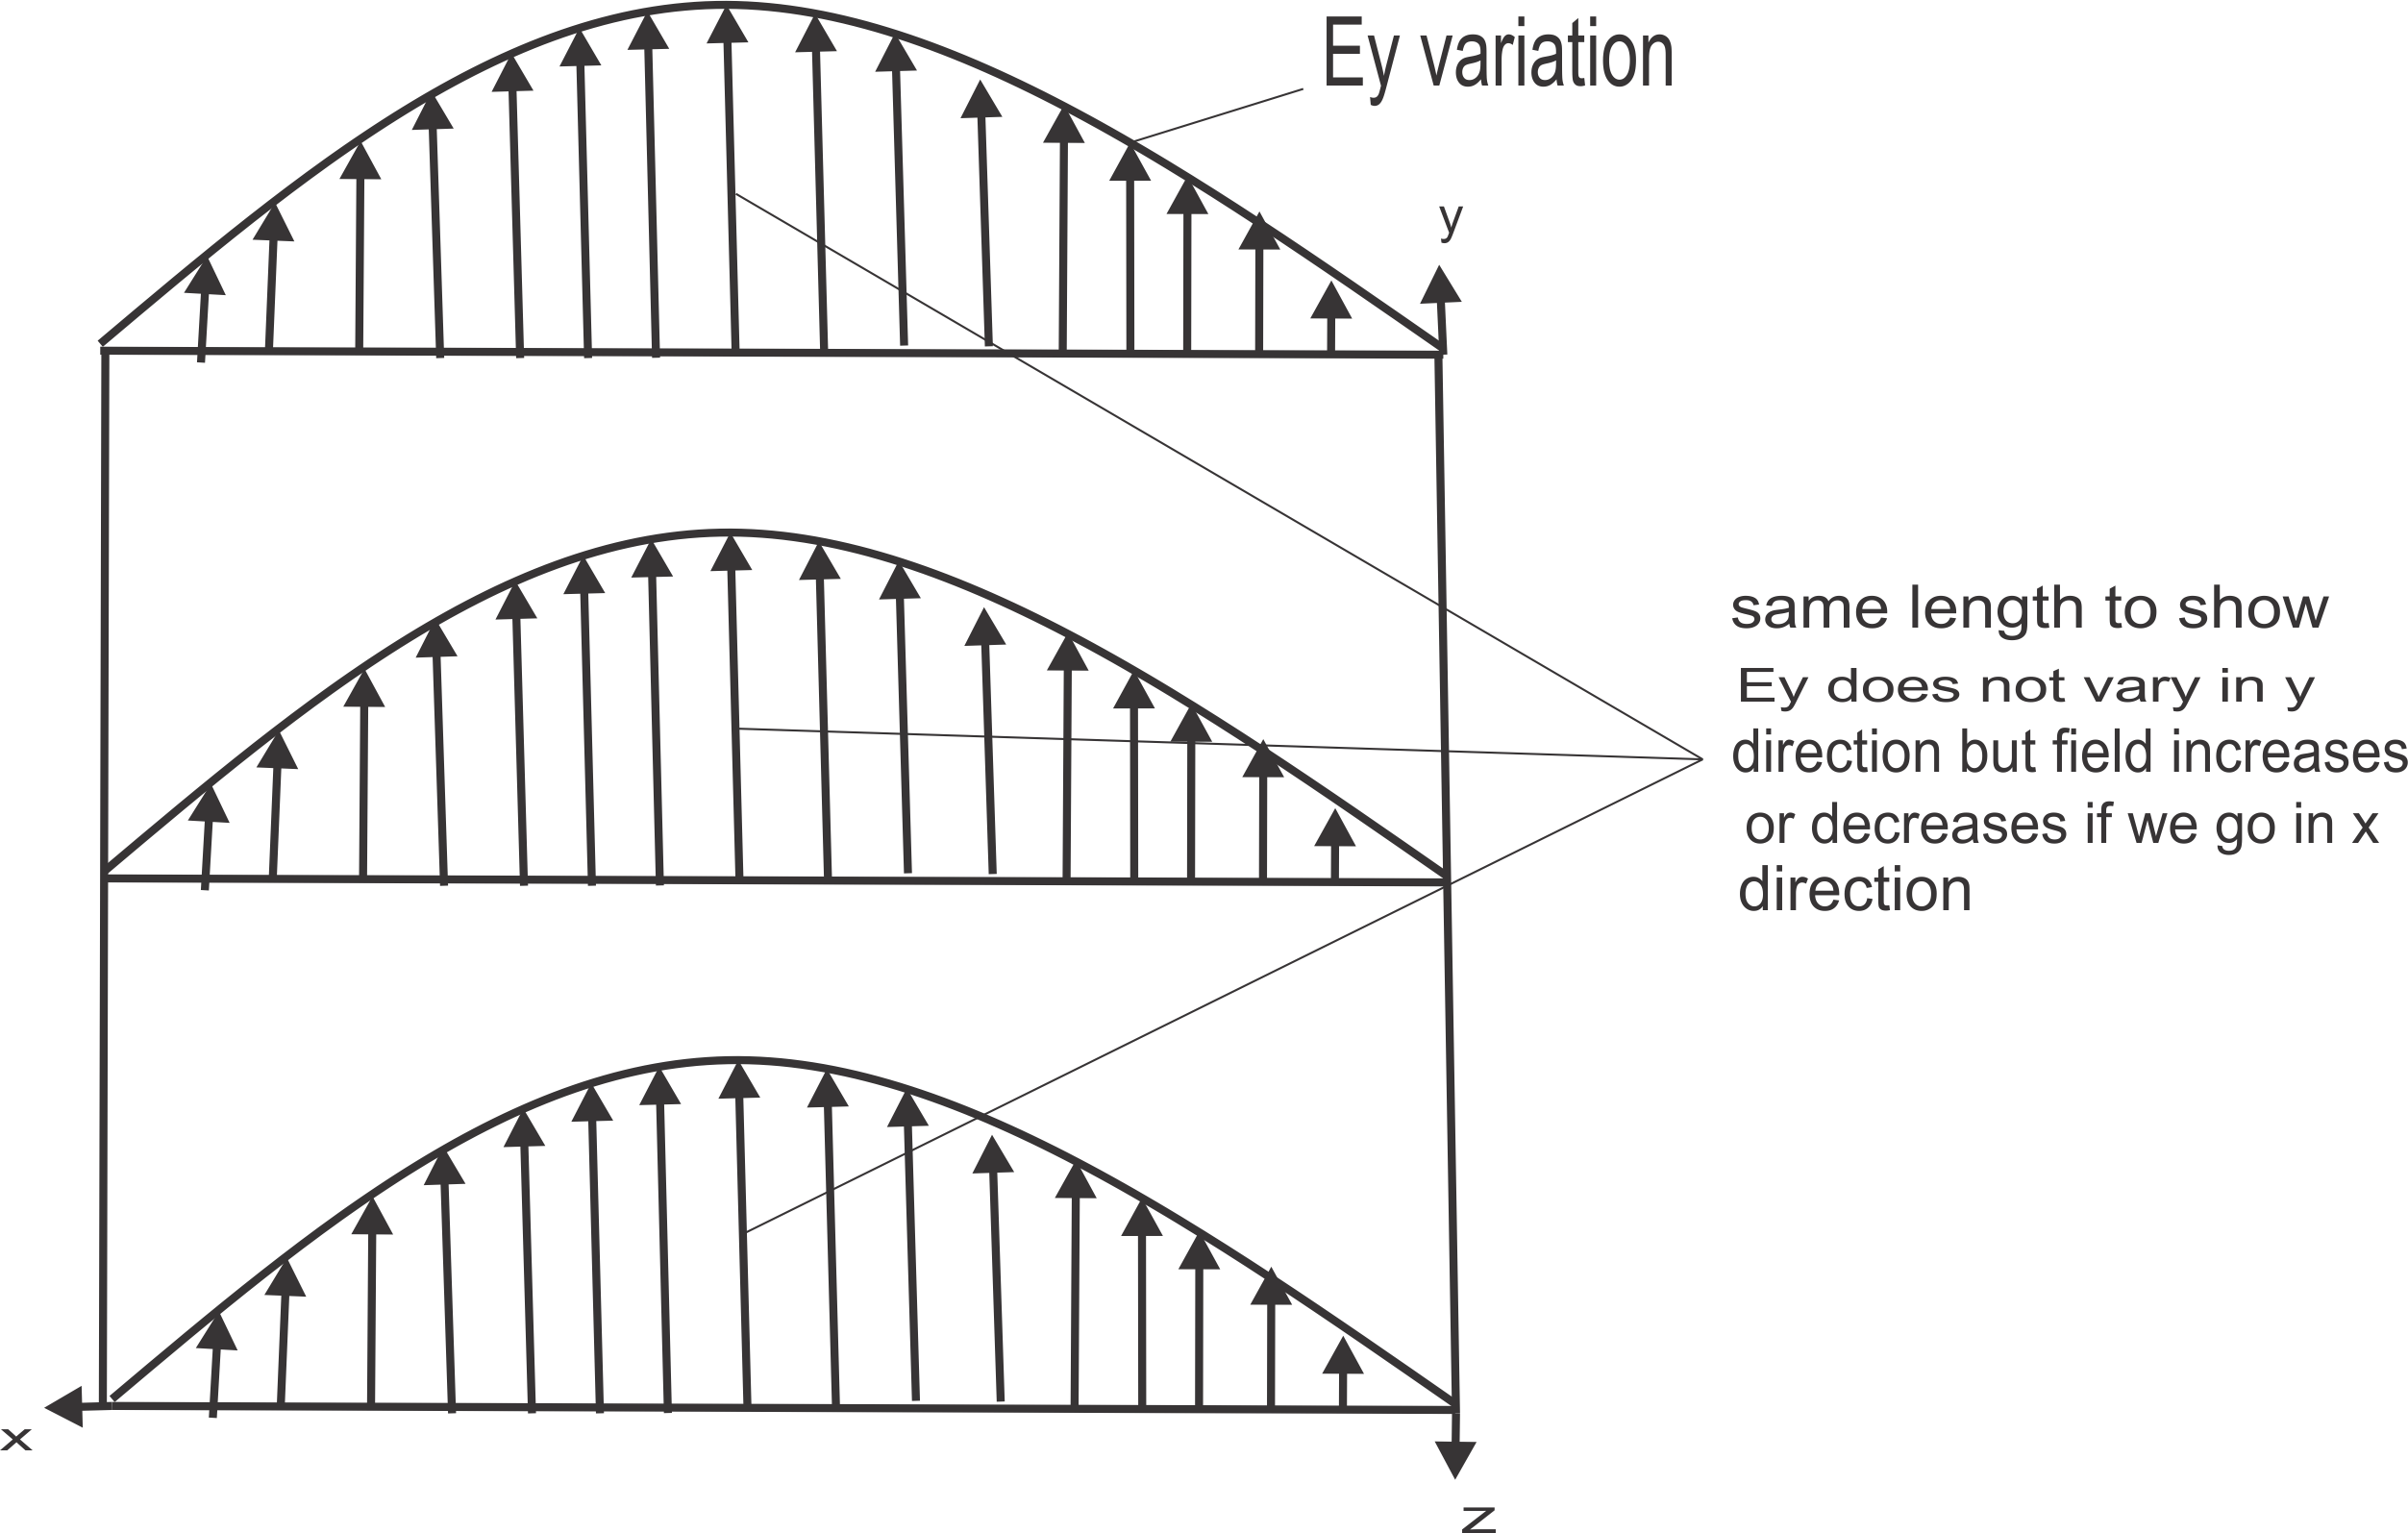
\includegraphics[width=1\linewidth]{\pathtoparttwo/graphics/group39-1}
\caption{Cross section of $E_y$ vector field in the dominant mode at an arbitrary value of z}
\label{fig:lec39-1}
\end{figure}

The field at a y-location is the same in magnitude and direction. However, it varies as we move in the x-direction, maximum at $x = 0$ and at $x = a$. The tangential components of $E_y$ against the side walls is equal to zero, we visualize the detail of these fields in different waveguiding structure later. At the moment, it appears $E_y$ is maximum at the broader wall of the waveguide as shown by the line traced on the waveguide in Figure~\ref{fig:lec39-2}. The same will happen to higher modes also you find the locations where the electric and magnetic fields are maximum. Why this information is important is one can ask a question that a waveguide is giving to you. How can a particular mode be excited inside the waveguide? Do we have a mechanism by which a particular order mode can be excited or can we selectively excite certain modes inside a waveguide?
\begin{figure}[h]
\centering
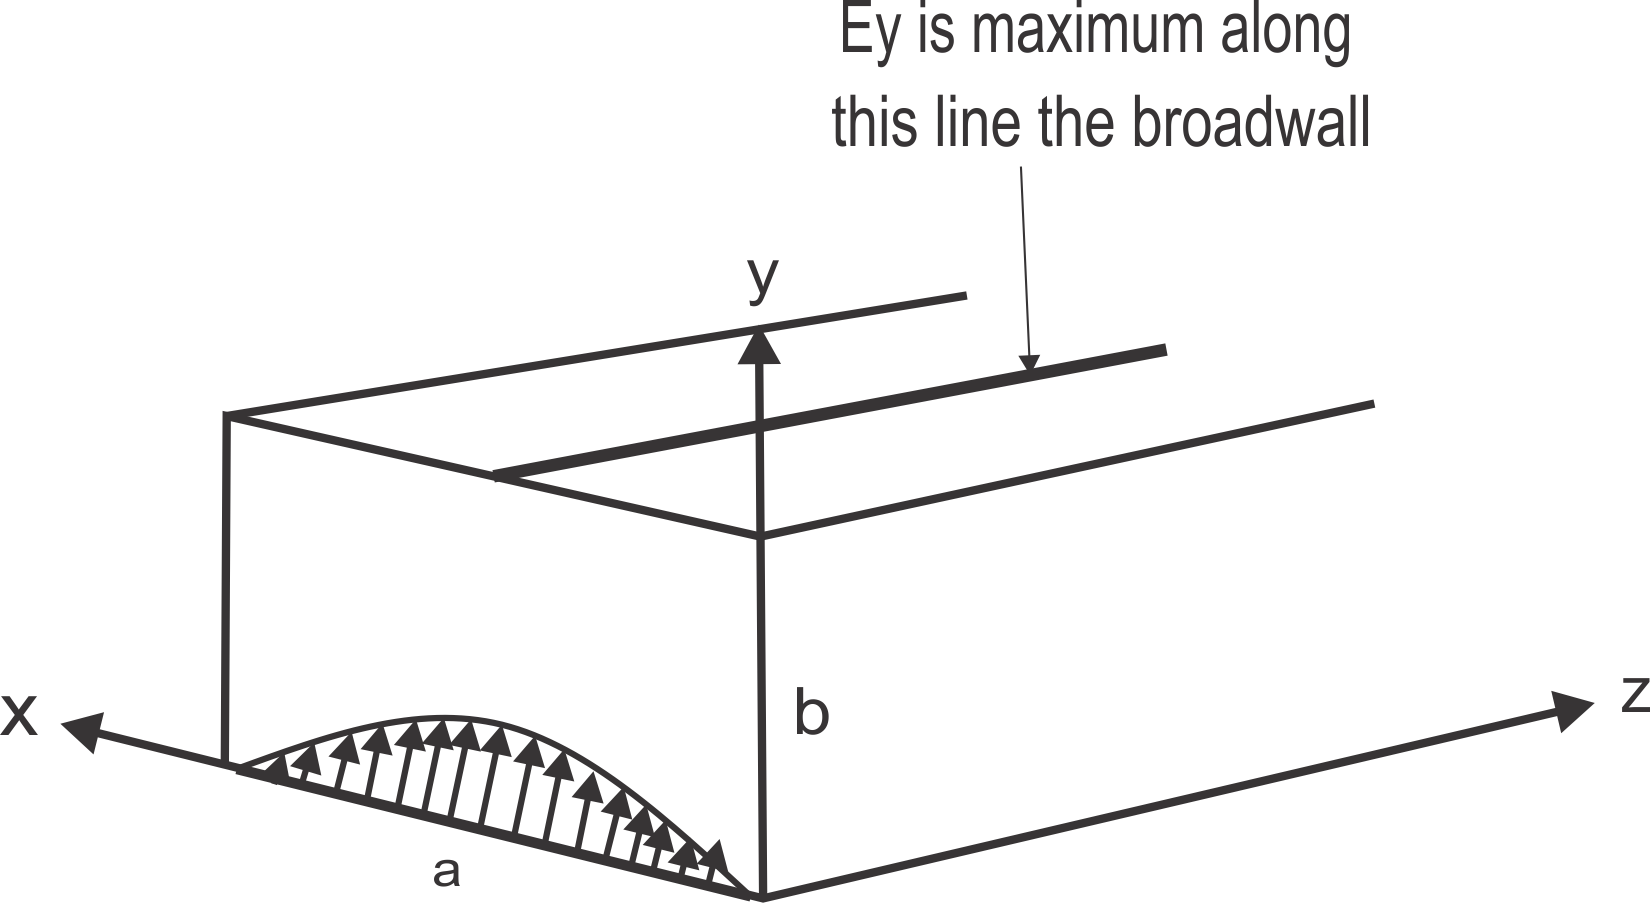
\includegraphics[width=1\linewidth]{\pathtoparttwo/graphics/group39-2}
\caption{Field pattern of $E_y$ along the z direction for the TE$_{10}$ mode}
\label{fig:lec39-2}
\end{figure}

By looking at the field distribution, it becomes clear that yes, if we create a mechanism by which the field is maximum along the line shown in Figure~\ref{fig:lec39-2} and as such the mode which will be excited inside the waveguide will be the TE$_{10}$ mode. So two things are required for excitation of this TE$_{10}$ mode, first, the size of the waveguide should be such that the x direction is broader than the y direction and second, the excitation mechanism should be such that the field or mode in which we want to get excited, matches with the excitation i.e maximum at the broader wall for the TE$_{10}$ mode in this case. So for the excitation of the TE$_{10}$ mode, we put some kind of a probe inside the waveguide on the broad wall and because of that, we have a finite field. For TE$_{10}$ mode, we talked about the field distribution satisfies the boundary conditions. We have the point of field excitation as shown in Figure~\ref{fig:lec39-3}, and then we show that to satisfy the boundary condition for a field, we require all possible modes for the waveguide either for travelling or decaying.
\begin{figure}[h]
\centering
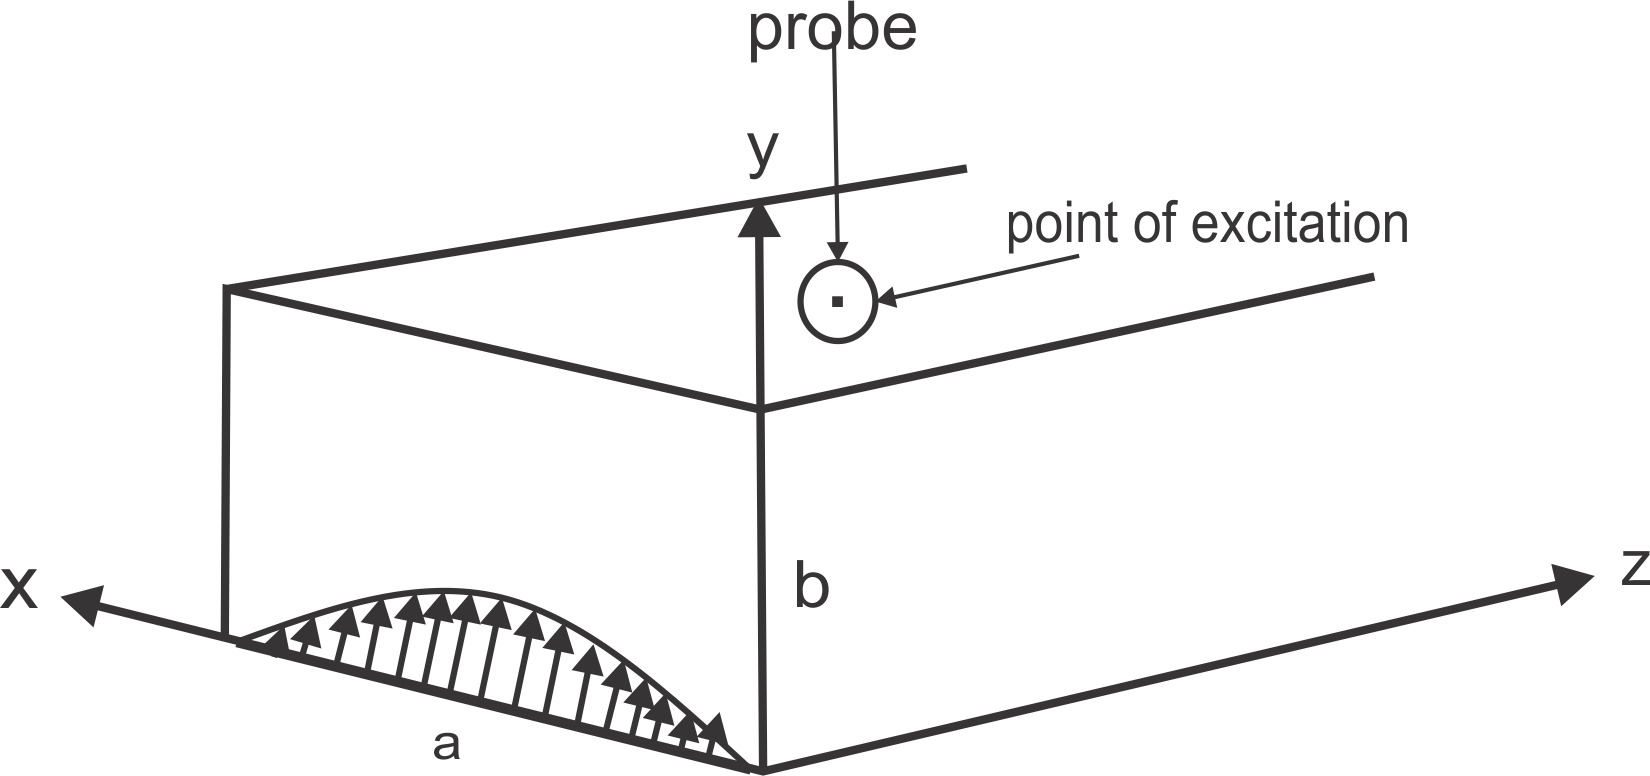
\includegraphics[width=1\linewidth]{\pathtoparttwo/graphics/group39-3}
\caption{Excitation of TE$_{10}$ mode}
\label{fig:lec39-3}
\end{figure}

These are essentially three orthogonal functions which satisfy the boundary condition inside the x structure. So locally around the probe, all kinds of modes get excited inside the waveguide, including the fields which are decaying fields. Only as we travel further in the waveguide, those fields which are below the cut-off will die down rapidly while only that frequency for which the cut-off frequency is less than will travel. If we make sure that this frequency is larger than the cut-off frequency of the TE$_{10}$ mode but smaller than any of the other cut-off frequencies, we get the TE$_{10}$ mode inside the waveguide structure guaranteed. So essentially a TE$_{10}$ mode inside the waveguide can be excited by pulling a probe which can excite an electric field inside the waveguide at the middle of the broader wall.

In practice, whenever we do the experiment, or we carry high-frequency signals like microwave signals, these signals are carried by a rectangular waveguide and this rectangular waveguide always operates in a mode which is the dominant mode of the waveguide called the TE$_{10}$ mode.

One can ask the question, how do we get the saying that we should operate this waveguide in a single-mode operation\index{single-mode operation or propagation}? There are many applications where we want a single-mode operation. The question is why we want a single-mode operation. The answer essentially lies in our dispersion relation. It says that the phase constant is a function of $m$ and $n$ i.e $\beta = \sqrt{{\omega}^2\mu\epsilon - \left(\dfrac{m\pi}{a}\right)^2 - \left(\dfrac{n\pi}{b}\right)^2}.$ Hence the velocity of the mode is a function of m and n. This means that for a given frequency $\omega$, the different modes are going to travel at different speeds. Now to send information on this waveguide, we try to put energy inside this waveguiding structure and then if larger modes can be supported by the waveguide structure when the waveguide is not in single mode operation, the energy will get distributed into various modes i.e various combinations of m and n. Each mode will have its velocity for travelling. So as it travels, the energy which is going on in different modes is essentially separated. Imagine a situation where we transmit signals which are not time-varying sinusoidal signals, say a pulse at high frequency, now if the energy is divided into different modes, and different modes travel at different speeds, then the energy reaches the other side of the waveguide, then all the modes will not reach the other end at the same time. That means the energy packet we send, will not be the energy packet we receive as they will be distributed in time as some modes will arrive earlier, and some modes will arrive later. So the dispersion phenomena we talk about essentially will give us the broadening of the signal in time as it travels on the waveguide. This is happening because energy is being distributed into various modes and different modes travel at different speeds. To avoid this, we try to put the energy only in one mode so that energy remains in that mode and the distribution of energy or differential delays which can be caused because of multiple modes of propagation inside the waveguide is avoided and we do not have a broadening of the signal when it travels on the waveguide, because of multi-mode propagation. This is the aspect one is to make use of when we design the waveguides at high frequencies.

In conclusion, for a rectangular waveguide, the important mode is the transverse electric mode TE$_{10}$ mode, that mode we also call dominant mode\index{dominant mode} because it has the lowest cut-off frequency and for this frequency, we should make sure single-mode propagation takes place over a certain range of frequencies. So in experiments, we make sure the frequency lies in that range so there is a single-mode propagation.

\section*{Exercises}
\begin{ExerciseList}
\Exercise[label={ex391}] 
What is the significance of the TE$_{10}$ mode in a rectangular waveguide, and why is it often referred to as the dominant mode?
\Exercise[label={ex392}]
What are the design requirements to excite TE$_{10}$ mode as a single-mode propagation
in a rectangular waveguide?
\Exercise[label={ex393}]
Why is single-mode operation desirable in waveguides, and how does it relate to the dispersion of signals?
\Exercise[label={ex394}]
Explain the concept of cut-off frequencies in the context of a rectangular waveguide. How do these frequencies depend on the dimensions of the waveguide?
\end{ExerciseList}
